\documentclass[12pt]{article}

\usepackage{amsmath,amsthm,amsfonts,amssymb,amsxtra}
\usepackage{multicol}
\usepackage{pgf,tikz}
\usetikzlibrary{arrows}
\renewcommand{\theenumi}{(\alph{enumi})} 
\renewcommand{\labelenumi}{\theenumi}

\pagestyle{empty}
\setlength{\textwidth}{7in}
\setlength{\oddsidemargin}{-0.5in}
\setlength{\topmargin}{-1.0in}
\setlength{\textheight}{9.5in}

\theoremstyle{definition}
\newtheorem{problem}{Problem}

\newcommand{\sectionlinetwo}[2]{%
  \nointerlineskip \vspace{.5\baselineskip}\hspace{\fill}
  {\color{#1}
    \resizebox{0.5\linewidth}{2ex}
    {{%
        {\begin{tikzpicture}
            \node  (C) at (0,0) {};
            \node (D) at (9,0) {};
            \path (C) to [ornament=#2] (D);
          \end{tikzpicture}}}}}%
  \hspace{\fill}
  \par\nointerlineskip \vspace{.5\baselineskip}
}

\makeatletter
\newcommand*{\radiobutton}{%
  \@ifstar{\@radiobutton0}{\@radiobutton1}%
}
\newcommand*{\@radiobutton}[1]{%
  \begin{tikzpicture}
    \pgfmathsetlengthmacro\radius{height("X")/2}
    \draw[radius=\radius] circle;
    \ifcase#1 \fill[radius=.6*\radius] circle;\fi
  \end{tikzpicture}%
}
\makeatother

\begin{document}

\noindent{\large\bf MATH 122}\hfill{\large\bf Exam \#1.}\hfill{\large\bf  Fall 2018}\hfill{\large\bf Page 1/8}\hrule

\bigskip
\begin{center}
  \begin{tabular}{|ll|}
    \hline & \cr
             {\bf Name: } & \makebox[12cm]{\hrulefill}\cr & \cr
                                                            {\bf VIP ID:} & \makebox[12cm]{\hrulefill}\cr & \cr
                                                                                                            \hline
  \end{tabular}
\end{center}
\begin{itemize}
\item Write your name and VIP ID in the space provided above.
\item The test has eight (8) pages, including this one.
\item Each question is worth 5 points. 
\item No books, or notes may be used on this test.
\item An approved calculator may be used on this test.
\end{itemize}
\hrule

\newpage

%%%%%%%%%%%%%%%%%%%%%%%%%%%%%%%%%%%%% Page 2
\noindent{\large\bf MATH 122}\hfill{\large\bf Exam \#1.}\hfill{\large\bf  Fall 2018}\hfill{\large\bf Page 2/8}\hrule

\bigskip
\begin{problem}[5 pts]
  The following table gives the sales of the medicinal herb \textit{saw palmetto}, in millions of dollars, for several
  different years: 
  \begin{center}
    \begin{tabular}{l||c|c|c|c|c|}
      Year & 1997 & 1998 & 1999 & 2000 & 2001 \\
      \hline
      Sales (million dollars) & 85 & 107 & 116 & 122 & 123
    \end{tabular}
  \end{center}
  The average rate of change of sales over the period 1997 to 2001 is:
  \begin{itemize}
  \item[\radiobutton] 123 million dollars/year
  \item[\radiobutton] 123 million dollars
  \item[\radiobutton] 38 million dollars/year
  \item[\radiobutton] 38 million dollars
  \item[\radiobutton] 9.5 million dollars/year
  \item[\radiobutton] 9.5 million dollars
  \item[\radiobutton] 4/38 million dollars/year
  \item[\radiobutton] 4/38 million dollars
  \end{itemize}
\end{problem}
\hrule

\begin{problem}[5 pts]
  You are to receive three equal payments of \$2000 each, paid once per year starting now. You can assume a 5\% interest
  rate, compounded continuously. The future value of the payments, on the day you receive the final payment, is: 
  \begin{itemize}
  \item[\radiobutton] $6000 e^{0.05 \cdot 3}$
  \item[\radiobutton] $6000 e^{0.05 \cdot 2}$
  \item[\radiobutton] $2000 e^{0.05 \cdot 3} + 2000 e^{0.05 \cdot 2} + 2000 e^{0.05 \cdot 1}$
  \item[\radiobutton] $2000 e^{0.05 \cdot 2} + 2000 e^{0.05 \cdot 1} + 2000$
  \end{itemize}
\end{problem}
\hrule

\begin{problem}[5 pts]
  The number of acres in a region cleared for farming follows the formula $A = f (t) = 2t^2$, where t is the number of
  months since the region started to be farmed and $t$ ranges from $t = 0$ to $t = 10$. Find the average rate of change in
  the number of acres cleared for farming between $t = 1$ and $t = 4$.  
  \begin{itemize}
  \item[\radiobutton] 10 acres/month
  \item[\radiobutton] 30 acres
  \item[\radiobutton] 10 months/acre
  \item[\radiobutton] 30 months
  \item[\radiobutton] 0.10 months/acre
  \end{itemize}
\end{problem}

\newpage

%%%%%%%%%%%%%%%%%%%%%%%%%%%%%%%%%%%%% Page 3
\noindent{\large\bf MATH 122}\hfill{\large\bf Exam \#1.}\hfill{\large\bf  Fall 2018}\hfill{\large\bf Page 3/8}\hrule

\bigskip
\begin{problem}[5 pts]
  The cost and revenue functions for a company are given by $C = 1000 + 3.75q$ and $R = 6.25q$.
  \begin{center}
    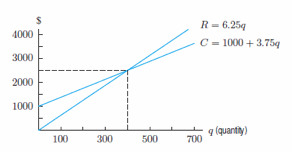
\includegraphics{1graph1.png}
  \end{center}
  The fixed costs of the company are:
  \begin{itemize}
  \item[\radiobutton] \$1,000 
  \item[\radiobutton] \$400
  \item[\radiobutton] \$0
  \item[\radiobutton] \$2,500
  \end{itemize}
\end{problem}
\hrule

\begin{problem}[5 pts]
  The cost in dollars to produce $q$ tons of an item is given by the cost function $C = 100 + 20q$. What are the units of
  the 20? 
  \begin{itemize}
  \item[\radiobutton] Dollars
  \item[\radiobutton] Tons
  \item[\radiobutton] Dollars/Tons
  \item[\radiobutton] Tons/Dollars
  \end{itemize} 
\end{problem}
\hrule

\begin{problem}[5 pts]
  The slope of the line connecting the points $(1, 4)$ and $(3, 8)$ is
  \begin{itemize}
  \item[\radiobutton] $-1/2$
  \item[\radiobutton] $-2$
  \item[\radiobutton] $1/2$
  \item[\radiobutton] $2$
  \end{itemize}
\end{problem}
\hrule

\begin{problem}[5 pts]
  It costs a total of $C$ dollars to extract $T$ tons of ore from a copper mine. If $C$ is a linear function of $T$, the
  units of the slope of the line are: 
  \begin{itemize}
  \item[\radiobutton] Tons
  \item[\radiobutton] Dollars
  \item[\radiobutton] Tons/dollar
  \item[\radiobutton] Dollars/ton
  \end{itemize}
\end{problem}

\newpage

%%%%%%%%%%%%%%%%%%%%%%%%%%%%%%%%%%%%% Page 4
\noindent{\large\bf MATH 122}\hfill{\large\bf Exam \#1.}\hfill{\large\bf Fall 2018}\hfill{\large\bf Page 4/8}\hrule

\bigskip
\begin{problem}[5 pts]
  The graph below is a representation of which of the following functions?
  \begin{multicols}{2}
    \begin{center}
      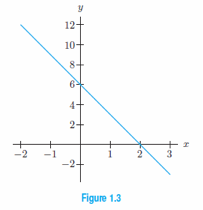
\includegraphics{1graph2.png}
    \end{center}
    \begin{itemize}
    \item[\radiobutton] $y=6x+6$
    \item[\radiobutton] $y=-3x+6$
    \item[\radiobutton] $y=-3x+2$
    \item[\radiobutton] $y=6x-2$
    \end{itemize}
  \end{multicols}
\end{problem}
\hrule

\begin{problem}[5 pts]
  When a person goes into shock, the cardiac output, in liters of blood per minute, decreases. One person’s cardiac output
  is 12 liters per minute when the person first goes into shock, and decreases by 2 liters per minute every hour that the
  person is in shock. Write a formula for cardiac output $C$ as a function of $t$, the time in hours since a person first
  went into shock. 
  \begin{itemize}
  \item[\radiobutton] $C = 12 - 2t$
  \item[\radiobutton] $t = 12 - 2C$
  \item[\radiobutton] $C = -2 + 12t$
  \item[\radiobutton] $t = -2 + 12t$
  \item[\radiobutton] $C = 12 + 2t$
  \item[\radiobutton] $t = 12 + 2C$
  \end{itemize}
\end{problem}
\hrule

\begin{problem}[5 pts]
  Assume $y = 100 - 2x$. If $x$ goes up by 3, the corresponding $y$--value changes by:
  \begin{itemize}
  \item[\radiobutton] $300$
  \item[\radiobutton] $-300$
  \item[\radiobutton] $6$
  \item[\radiobutton] $-6$
  \item[\radiobutton] $94$
  \item[\radiobutton] $-94$
  \end{itemize} 
\end{problem}

\newpage

%%%%%%%%%%%%%%%%%%%%%%%%%%%%%%%%%%%%% Page 5
\noindent{\large\bf MATH 122}\hfill{\large\bf Exam \#1.}\hfill{\large\bf  Fall 2018}\hfill{\large\bf Page 5/8}\hrule

\bigskip

\begin{problem}[5 pts]
  The amount, $A$ (in mg), of a drug in the body is 25 when it first enters the system is decreases by 12\% each hour. A
  possible formula for $A$ as a function of $t$, in hours after the drug enters the system, is: 
  \begin{itemize}
  \item[\radiobutton] $A= 25+12t$
  \item[\radiobutton] $A=25-12t$
  \item[\radiobutton] $A=25+0.12t$
  \item[\radiobutton] $A=25-0.12t$
  \item[\radiobutton] $A=25(0.12)^t$
  \item[\radiobutton] $A=25(0.88)^t$
  \item[\radiobutton] $A=25(1.12)^t$
  \item[\radiobutton] $A=25(1.88)^t$
  \item[\radiobutton] $A=25(-0.12)^t$
  \end{itemize}
\end{problem}

\vspace{1cm}
\hrule

\begin{problem}[5 pts]
  Indicate whether the following are power functions. In case they are, find a suitable constant of proportionality $k$,
  and power $p$ so you could write those functions in the form $f(x) = kx^p$. 
  \begin{center}
    \begin{tabular}{|c|c|c|c|}
      \hline
      $f(x)$ & power function? & $k$ & $p$ \\
      \hline
      \hline
             &&& \\
      $5\sqrt{x}$ &&\hspace{1cm} & \hspace{1cm} \\
             &&& \\
      \hline
             &&& \\
      $17^x$ &&& \\
             &&& \\
      \hline
             &&& \\
      $(3x^5)^2$ &&& \\
             &&& \\
      \hline
             &&& \\
      $\dfrac{5}{2\sqrt{x}}$ &&& \\
             &&& \\
      \hline
             &&& \\
      $\pi$ &&& \\
             &&& \\
      \hline
    \end{tabular}
  \end{center}
\end{problem}
\newpage


%%%%%%%%%%%%%%%%%%%%%%%%%%%%%%%%%%%%% Page 6
\noindent{\large\bf MATH 122}\hfill{\large\bf Exam \#1.}\hfill{\large\bf  Fall 2018}\hfill{\large\bf Page 6/8}\hrule

\bigskip

\begin{problem}[5 pts]
  Given the graph of the function $f(x)$ below (left), sketch the graph of the function $2-f(2x)$. 
  \begin{center}
    \begin{tikzpicture}[scale=2]
      \draw[step=0.25, help lines] (-2,-2) grid (2,2);
      \draw[ultra thick](0,-2)--(0,2);
      \draw[ultra thick](-2,0)--(2,0);
      \foreach \x in {-2,-1.75,-1.5,...,2}{
        \draw (-0.1,\x)--(0.1,\x);
        \draw (\x, -0.1)-- (\x, 0.1);
      }
      \draw[blue,ultra thick](-2,0.5)--(-1,1)--(0,0)--(1,1)--(2,1);

      \begin{scope}[xshift=5cm]
        \draw[step=0.25, help lines] (-2,-2) grid (2,2);
        \draw[ultra thick](0,-2)--(0,2);
        \draw[ultra thick](-2,0)--(2,0);
        \foreach \x in {-2,-1.75,-1.5,...,2}{
          \draw (-0.1,\x)--(0.1,\x);
          \draw (\x, -0.1)-- (\x, 0.1);
        }
      \end{scope}
    \end{tikzpicture}
  \end{center}  
\end{problem}

\vspace{2cm}
\hrule

\begin{problem}[5 pts]
  The solution to $200 = 30e^{0.15t}$ is:
  \begin{itemize}
  \item[\radiobutton] $t = \dfrac{\ln(200/30)}{\ln(0.15)}$
  \item[\radiobutton] $t = \dfrac{\ln(200/30)}{0.15}$
  \item[\radiobutton] $t = \ln \bigg(\dfrac{200}{30 (0.15)} \bigg)$
  \item[\radiobutton] $t = \frac{200}{30}\ln(0.15)$
  \end{itemize}
\end{problem}
\hrule

\begin{problem}[5 pts]
  The average rate of change of sales of the medicinal herb \textit{saw palmetto} in the US during the period 1997 to 2001
  is 9.5 million dollars per year. This means that, during the years 1997 to 2001, in the US: 
  \begin{itemize}
  \item[\radiobutton] Sales of \textit{saw palmetto} averaged 9.5 million dollars each year.
  \item[\radiobutton] Sales of \textit{saw palmetto} increased by an average of 9.5 million dollars each year.
  \item[\radiobutton] Sales of \textit{saw palmetto} were 9.5 million dollars in each of the years.
  \item[\radiobutton] Sales of \textit{saw palmetto} went up by 9.5 million dollars in each of the years.
  \end{itemize}
\end{problem}

\newpage 


%%%%%%%%%%%%%%%%%%%%%%%%%%%%%%%%%%%%% Page 7
\noindent{\large\bf MATH 122}\hfill{\large\bf Exam \#1.}\hfill{\large\bf  Fall 2018}\hfill{\large\bf Page 7/8}\hrule

\bigskip
\begin{problem}[5 pts]
  Converting the function $P = 100 (1.07)^t$ to the form $P = P_0e^{kt}$ gives
  \begin{itemize}
  \item[\radiobutton] $P = 100e^{1.07t}$
  \item[\radiobutton] $P = 100 e^{0.07t}$
  \item[\radiobutton] $P = 100 e^{1.0677t}$
  \item[\radiobutton] $P = 100 e^{0.0677t}$
  \item[\radiobutton] $P = 100 e^{0.93t}$
  \end{itemize}
\end{problem}

\hrule

\begin{problem}[5 pts]
  Converting the function $P = 750e^{0.04t}$ to the form $P = P_0a^t$ gives
  \begin{itemize}
  \item[\radiobutton] $P = 750 (1.04)^t$
  \item[\radiobutton] $P = 750 (0.04)^t$
  \item[\radiobutton] $P = 750 (1.0408)^t$
  \item[\radiobutton] $P = 750 (0.0408)^t$
  \item[\radiobutton] $P = 750 (0.96)^t$
  \end{itemize}
\end{problem}
\hrule

\begin{problem}[5 pts]
  The concentration of a pollutant in a lake is 85 parts per million (ppm) and is increasing at a rate of 4.6\% each
  year. A possible formula for the concentration $C$ as a function of year $t$ is: 
  \begin{itemize}
  \item[\radiobutton] $C = 85 + 4.6t$
  \item[\radiobutton] $C = 85 - 4.6t$
  \item[\radiobutton] $C = 85 + 0.046t$
  \item[\radiobutton] $C = 85 - 0.046t$
  \item[\radiobutton] $C = 85(0.046)^t$
  \item[\radiobutton] $C = 85(0.954)^t$
  \item[\radiobutton] $C = 85(1.046)^t$
  \item[\radiobutton] $C = 85(1.46)^t$
  \item[\radiobutton] $C = 85(0.46)^t$
  \item[\radiobutton] $C = 46(0.85)^t$
  \end{itemize}
\end{problem}
\newpage

%%%%%%%%%%%%%%%%%%%%%%%%%%%%%%%%%%%%% Page 8
\noindent{\large\bf MATH 122}\hfill{\large\bf Exam \#1.}\hfill{\large\bf  Fall 2018}\hfill{\large\bf Page 8/8}\hrule

\bigskip
\begin{problem}[5 pts]
  Sales at a company are changing according to the formula $S = 1000 (0.82)^t$ , where $S$ is sales in thousands of
  dollars and $t$ is measured in years. Sales at this company are: 
  \begin{itemize}
  \item[\radiobutton] Increasing by 82\% per year
  \item[\radiobutton] Increasing by 82 thousand dollars per year
  \item[\radiobutton] Decreasing by 82\% per year
  \item[\radiobutton] Decreasing by 82 thousand dollars per year
  \item[\radiobutton] Increasing by 18\% per year
  \item[\radiobutton] Increasing by 18 thousand dollars per year
  \item[\radiobutton] Decreasing by 18\% per year
  \item[\radiobutton] Decreasing by 18 thousand dollars per year
  \end{itemize} 
\end{problem}
\hrule

\begin{problem}[5 pts]
  The number $N$ of species of reptiles found on an island is proportional to the fourth root of the area of the island,
  $A$.  Which of the following represents this statement? 
  \begin{itemize}
  \item[\radiobutton] $N=A^{1/4}$
  \item[\radiobutton] $A=N^{1/4}$
  \item[\radiobutton] $N=A^{-4}$
  \item[\radiobutton] $A=N^{-4}$
  \item[\radiobutton] $N=kA^{1/4}$
  \item[\radiobutton] $A=kN^{1/4}$
  \item[\radiobutton] $N=kA^{-4}$
  \item[\radiobutton] $A=kN^{-4}$
  \end{itemize}
\end{problem}

\end{document}
